%%MAIN: thesis.tex

%%%%% The Validation %%%%%
\chapter{Implementation: Lesson Plans} \label{ch_teaching}
% formerly: Teaching with \texttt{PA}
In its current form, \texttt{Processing Abstractions} as presented in chapter \ref{ch_pa} is mainly targetted at the obligatory introduction to computer sciences at high school level.

Before going into empirical results from using \texttt{PA} in two courses, three lesson plans will be presented for which \texttt{PA} has been developed: a \emph{Sichtenwechsel} in computer architecture (section \ref{sc_lesson_ca}); an introduction into the inner workings of a compiler (section \ref{sc_lesson_compiler}); and a plan for a general introduction to programming (section \ref{sc_lesson_intro}). Some ideas for how to expand it for other school levels will be presented in section \ref{sc_lesson_other}.

For all the lessons, students will need a local environment of \texttt{Processing Abstractions} installed on a computer available to them. See appendix \ref{ch_setup} for how to set it up. Additionally, for non-German speaking students the contents will have to be translated to the teaching language.

\section{Lesson on Computer Architecture} \label{sc_lesson_ca}
% Using PA to demonstrate what happens under the hood when running a program in a high level language.
Introductions to computer science which extend beyond a pure programming course often contain lessons on computer architecture. E.\,g. the curriculum \cite[p.\,145]{Erz16} asks for students to ``know how computers and networks are structured and work''.

Now a sequence of lessons on the subject might be ordered either bottom up (as elaborated in subsection \ref{ssc_bottom_up}) or top down (\ref{ssc_top_down}). In either case, this proposed lesson will go towards the middle or can be used at the end as part of a repetition sequence.

\subsection{Prerequisites}
Students must already know basic programming skills in a high level language such as Processing (see section \ref{sc_processing}). In particular, they must know about variables and loops. An introduction to programming could also be done using \texttt{PA} as outlined in \ref{sc_lesson_intro} below.

The more students are supposed to work on their own, the more they'll need an overview over the different layers prior to combining them. As a prerequisite, it it recommended to at least introduce the Von Neumann architecture and its split of the CPU into control unit and arithmetic unit:

\begin{center}
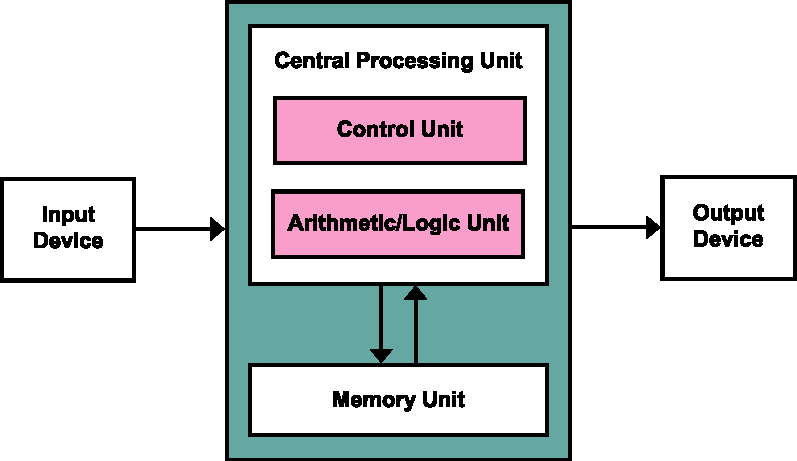
\includegraphics[width=10cm]{images/Von_Neumann_Architecture.pdf}
\\ \xxx{replace or properly attribute: Kapooht, 2013, CC BY-SA 3.0}
\end{center}

In a bottom up approach, this might also include the introduction of transistors, logic gates and circuits. In a top down approach, these could also be treated afterwards.

\subsection{Lesson Plan}
The goal of the lesson is for students to have connected their knowledge of high level programming with what happens within their machine when a program is executed.

If this is the student's encounter with Glamorous Toolkit, at least a brief introduction is in order (see \ref{ssc_lesson_gt}). Else we can directly start with a reminder of what they already know about programming.


\section{Lesson on Compilers} \label{sc_lesson_compiler}
Using PA to demonstrated the steps of lexing, parsing, transpiling, compiling and optimizing.

\section{Introduction to Programming} \label{sc_lesson_intro}
Using PA as a live programming environment.

\subsection{Introduction to Glamorous Toolkit} \label{ssc_lesson_gt}

\section{Further Lesson Ideas} \label{sc_lesson_other}
Connecting PA with Smalltalk; extend it to object oriented programming; mould the environment to questions developed during the course; ...

\chapter{Validation} \label{ch_practice}
% formerly: \texttt{PA} in Practice
PA has been used twice with students (on 2025-05-12 and 2025-06-30).

\section{First Round}
\subsection{Setting}
\subsection{Observations}
\subsection{Student Feedback}
\subsection{Learnings}

\section{Second Round}
\subsection{Setting}
\subsection{Observations}
\subsection{Student Feedback}
\subsection{Learnings}
